% Appendix template for Major Project Report (2026-27)
% Include only appendices relevant to the project. Replace all guidance text.

\begin{appendices}

\chapter{Project Planning}

\section{Project Timeline}
Provide the project schedule, milestones, task allocation, and timeline. Insert the project Gantt chart or schedule figure below.

\subsection{Project Timeline}

The project timeline illustrates the planned phases of project development,
including requirement analysis, literature survey, design, implementation,
testing, validation, and documentation.

\begin{figure}[htbp]
	\centering
	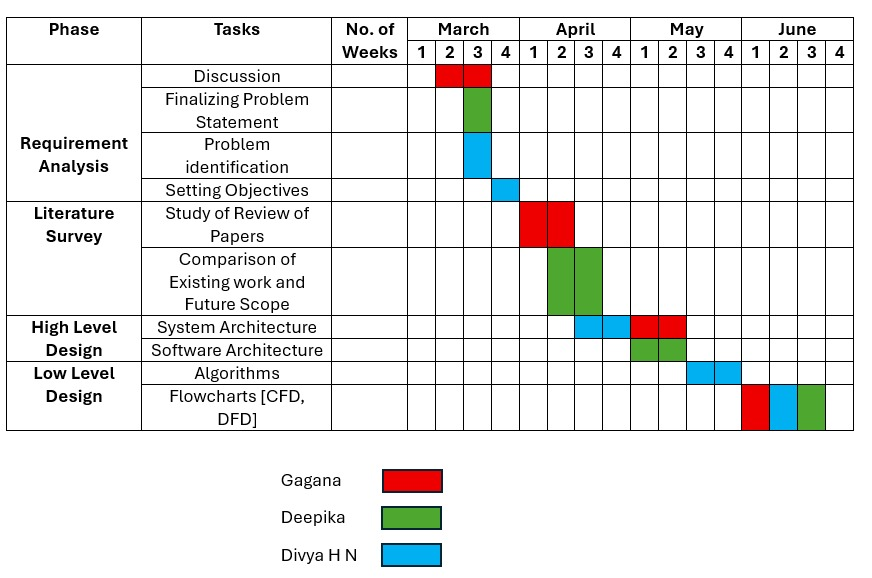
\includegraphics[width=\textwidth]{timeline}
	\caption{Project Timeline}
	\label{fig:project-timeline}
\end{figure}
% Example:
% \begin{figure}[htbp]
%   \centering
%   \includegraphics[width=\textwidth]{project_timeline.png}
%   \caption{Project Timeline}
%   \label{fig:project-timeline}
% \end{figure}

\section{Budget Estimation}
Describe the hardware, software, services, and other resources used, and provide a cost estimate.

\begin{figure}[htbp]
	\centering
	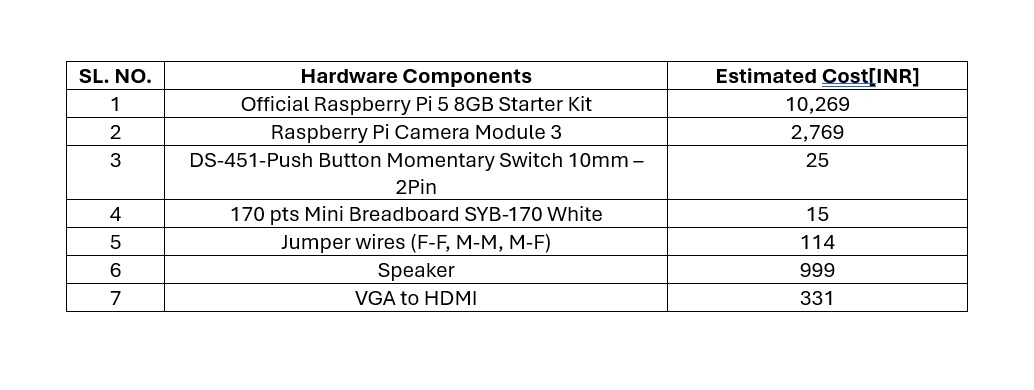
\includegraphics[width=\textwidth]{budget}
	\caption{Project Budget}
	\label{fig:project-budget}
\end{figure}

% Example budget table (edit as required):
% \begin{table}[htbp]
% \centering
% \caption{Estimated Project Budget}
% \begin{tabular}{|l|r|}\hline
% Item & Estimated Cost (INR) \\ \hline
% Hardware & 0 \\ Software & 0 \\ Other expenses & 0 \\ \hline
% Total & 0 \\ \hline
% \end{tabular}
% \end{table}

\chapter{Sustainable Development Goals (SDGs) Addressed}
Explain how the project contributes to relevant Sustainable Development Goals (SDGs). Include an SDG mapping table, define the rating scale used, and provide a short justification for each SDG selected. Include only SDGs with a meaningful project contribution.

\begin{table}[htbp]
	\centering
	\caption{SDG Impact Evaluation}
	\label{tab:sdg-impact}
	\begin{tabular}{|p{10cm}|c|}
		\hline
		\textbf{Sustainable Development Goal} & \textbf{Level} \\
		\hline
		No Poverty & 1 \\ \hline
		Zero Hunger & 1 \\ \hline
		Good Health and Well-being & 2 \\ \hline
		Quality Education & 2 \\ \hline
		Gender Equality & 1 \\ \hline
		Clean Water and Sanitation & 1 \\ \hline
		Affordable and Clean Energy & 1 \\ \hline
		Decent Work and Economic Growth & 2 \\ \hline
		Industry, Innovation and Infrastructure & 3 \\ \hline
		Reduced Inequalities & 2 \\ \hline
		Sustainable Cities and Communities & 3 \\ \hline
		Responsible Consumption and Production & 1 \\ \hline
		Climate Action & 1 \\ \hline
		Life Below Water & 1 \\ \hline
		Life on Land & 1 \\ \hline
		Peace, Justice and Strong Institutions & 3 \\ \hline
		Partnerships for the Goals & 3 \\ \hline
	\end{tabular}
\end{table}

\noindent\textbf{Levels:} Poor = 1, Good = 2, Excellent = 3.

\subsection{SDGs with the Highest Contribution}

The project demonstrates a strong contribution to four Sustainable Development
Goals (SDGs), namely SDG 9 (Industry, Innovation and Infrastructure),
SDG 11 (Sustainable Cities and Communities), SDG 16 (Peace, Justice and
Strong Institutions), and SDG 17 (Partnerships for the Goals), each
assigned a contribution level of 3 (Excellent).

\textbf{SDG 9: Industry, Innovation and Infrastructure:}
The project contributes to strengthening digital infrastructure by developing
an effective cybersecurity solution for detecting malicious activities in
encrypted network traffic. The use of advanced machine learning models and
modern computing technologies supports innovation and enhances the resilience
of digital infrastructure.

\textbf{SDG 11: Sustainable Cities and Communities:}
The project supports secure digital environments that are essential for smart
cities and connected communities. Detecting malicious activities in encrypted
network traffic can help protect digital services, public networks, and
connected infrastructure, thereby contributing to safer and more reliable
digital ecosystems.

\textbf{SDG 16: Peace, Justice and Strong Institutions:}
The proposed solution strengthens cybersecurity by helping identify covert
communication and potential data exfiltration activities. This supports the
security, reliability, and trustworthiness of digital systems used by
institutions and organizations.

\textbf{SDG 17: Partnerships for the Goals:}
The project promotes collaboration and knowledge sharing through the use of
open-source tools, publicly available datasets, and reproducible research
methodologies. The integration of technologies from networking,
cybersecurity, machine learning, and software engineering demonstrates
the value of interdisciplinary collaboration in addressing cybersecurity
challenges.

\chapter{Self-Assessment of the Project}
The project was evaluated against the Program Outcomes (POs) and
Program Specific Outcomes (PSOs) to assess the extent to which the
engineering knowledge, technical skills, problem-solving abilities,
professional practices, and project management capabilities were
demonstrated during the project development process.
The assessment reflects the contribution of the project towards
achieving the defined graduate attributes and program-specific
competencies. The contribution levels are categorized as Poor (1),
Good (2), and Excellent (3).

\section{Self-Assessment of the Project}

\begin{longtable}{|c|p{5.2cm}|p{7cm}|c|}
	\caption{Self-Assessment of the Project Outcomes}
	\label{tab:self-assessment}\\
	\hline
	\textbf{No.} & \textbf{PO and PSO} & \textbf{Contribution from the Project} & \textbf{Level} \\
	\hline
	\endfirsthead
	
	\hline
	\textbf{No.} & \textbf{PO and PSO} & \textbf{Contribution from the Project} & \textbf{Level} \\
	\hline
	\endhead
	
	1 &
	Engineering Knowledge &
	Applied concepts of mathematics, computer networks, cybersecurity,
	machine learning, deep learning, and computer engineering to design
	and implement the proposed system. &
	3 \\ \hline
	
	2 &
	Problem Analysis &
	Identified limitations of existing approaches, reviewed research literature,
	analyzed the challenges associated with the problem, and formulated an
	effective solution. &
	3 \\ \hline
	
	3 &
	Design and Development of Solutions &
	Designed and developed a system architecture, processing pipeline,
	model architecture, and software components to address the identified
	problem. &
	3 \\ \hline
	
	4 &
	Conduct Investigations of Complex Problems &
	Conducted experiments, evaluated models, analyzed datasets, performed
	parameter tuning, and interpreted results using appropriate performance
	metrics. &
	3 \\ \hline
	
	5 &
	Modern Tool Usage &
	Utilized appropriate programming languages, libraries, frameworks,
	software tools, and computing platforms to develop, test, and evaluate
	the proposed system. &
	3 \\ \hline
	
	6 &
	The Engineer and the World &
	Considered the societal, environmental, economic, and practical
	implications of the proposed engineering solution and its deployment. &
	2 \\ \hline
	
	7 &
	Ethics &
	Followed responsible engineering and research practices, considered
	ethical aspects of data usage, and maintained responsible handling
	of project information. &
	3 \\ \hline
	
	8 &
	Individual and Team Work &
	Worked independently and collaboratively in planning, implementing,
	integrating, testing, and completing the project activities. &
	3 \\ \hline
	
	9 &
	Communication &
	Presented technical information and project outcomes through
	documentation, reports, presentations, diagrams, and other
	project artifacts. &
	3 \\ \hline
	
	10 &
	Project Management and Finance &
	Planned project activities, managed available resources, followed
	development milestones, and considered implementation costs
	and resource utilization. &
	3 \\ \hline
	
	11 &
	Life-long Learning &
	Learned and applied new technologies, tools, algorithms, and
	technical concepts beyond the prescribed curriculum to solve
	the identified engineering problem. &
	3 \\ \hline
	
	12 &
	PSO1 -- Computer-Based Systems Development &
	Applied knowledge of computing systems, operating systems,
	computer architecture, and related technologies in developing
	the proposed system. &
	3 \\ \hline
	
	13 &
	PSO2 -- Software Development &
	Developed software components and applications using
	programming languages, algorithms, data structures,
	software engineering practices, and appropriate tools. &
	3 \\ \hline
	
	14 &
	PSO3 -- Computer Communications and Internet Applications &
	Applied knowledge of computer networks, communication protocols,
	and Internet technologies in designing and implementing
	the proposed system. &
	3 \\ \hline
	
\end{longtable}

\noindent\textbf{Levels:} Poor = 1, Good = 2, Excellent = 3.




\chapter{Input Details}
\section{Dataset / Input Details}
Document the datasets, inputs, data sources, collection procedures, composition, labels, relevant features, and preprocessing steps. Include only details relevant to the project.

\section{Data Collection / Capture Methodology}
Describe the tools, procedures, setup, and filters used to collect or generate input data, where applicable.

\section{Input Features and Label Encoding}
List and explain the input features and the encoding or labeling scheme used, where applicable.

\chapter{Configuration Details}
\section{System Requirements}
Specify the minimum and recommended hardware requirements, including processor, memory, storage, and other project-specific requirements.

\section{Software Configuration}
List the operating system, development tools, libraries, frameworks, software versions, and supporting utilities used.

\section{Model and System Configuration}
Describe the relevant model parameters, architecture, system settings, deployment configuration, and workflow settings.

\section{Evaluation Metrics}
Define the evaluation metrics used and briefly state why they are appropriate for the project.

\section{GitHub Repository}
Provide the public GitHub repository URL for the source code and project artifacts. Ensure the repository includes an appropriate README.

% Add further appendices only when necessary, using additional \chapter commands.

\end{appendices}
